%-----------------------------------------------------------------------------
%	PACKAGES AND DOCUMENT CONFIGURATIONS
%-----------------------------------------------------------------------------

\documentclass{article}

\usepackage{graphicx} % Required for the inclusion of images
\usepackage{natbib} % Required to change bibliography style to APA
\usepackage{amsmath} % Required for some math elements
\usepackage{mathtools}
\usepackage{grffile}
\usepackage[export]{adjustbox}
\usepackage{subcaption}
\usepackage{float}
\usepackage{listings}
\usepackage[margin=1.0in]{geometry}
\usepackage{tikz}
\usepackage{enumitem}
\usepackage{scrextend}
\usepackage{siunitx}

\usetikzlibrary{shapes.geometric, arrows}
\tikzstyle{startstop} = [rectangle, rounded corners, minimum width=1cm, minimum height=1cm,text centered, draw=black, fill=white!30]
\tikzstyle{process} = [rectangle, minimum width=1cm, minimum height=1cm, text centered, draw=black, fill=white!30]
\tikzstyle{arrow} = [thick,->,>=stealth]

\DeclarePairedDelimiter{\abs}{\lvert}{\rvert}
\setlength\parindent{0pt} % Removes all indentation from paragraphs

%-----------------------------------------------------------------------------
%	DOCUMENT INFORMATION
%-----------------------------------------------------------------------------

\title{ECE 547 Fall 2016 Homework 1} % Title

\author{Yang \textsc{Wang}} % Author name

\date{\today} % Date for the report

\renewcommand{\theenumi}{\alph{enumi}} % use letters for list items

\begin{document}

\maketitle % Insert the title, author and date

%-----------------------------------------------------------------------------
%	Problem 1
%-----------------------------------------------------------------------------

\section*{Problem 1}
	In this problem, \textbf{CP} stands for Calling Party. \textbf{CDP} stands for
	Called Party and \textbf{TN} stands for Telephone Network.
	\begin{enumerate}
		\item Call display (Caller ID): \textbf{CP} initiates the call. \textbf{TN}
			perform circuit-switching and connects the \textbf{CP} to the \textbf{CDP}.
			During the initial stage of the connection, \textbf{TN} retrieve and send
			data in regard to the identification (location, name, etc) of the \textbf{CP}
			to the \textbf{CDP}. The following diagram summarizes this process:

			\begin{figure}[hbt]
				\centering
					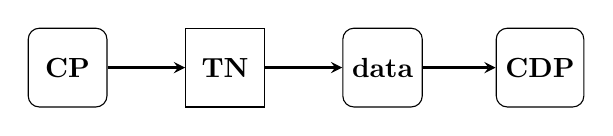
\begin{tikzpicture}[node distance=2cm]
						\node (cp) [startstop] {\textbf{CP}};
						\node (tn) [process, right of=cp] {\textbf{TN}};
						\node (data) [startstop, right of=tn] {\textbf{data}};
						\node (cdp) [startstop, right of=data] {\textbf{CDP}};
						\draw [arrow] (cp) -- (tn);
						\draw [arrow] (tn) -- (data);
						\draw [arrow] (data) -- (cdp);
					\end{tikzpicture}
				\caption{Call display diagram}
			\end{figure}
		\item Calling waiting: when the second \textbf{CP} attempts calling the \textbf{CDP},
			the \textbf{TN} could issue a beep sound to the \textbf{CDP} and remain
			the existing connection. It could be summarized as this diagram:

			\begin{figure}[hbt]
				\centering
					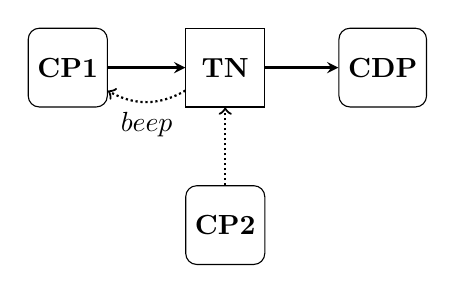
\begin{tikzpicture}[node distance=2cm]
						\node (cp1) [startstop] {\textbf{CP1}};
						\node (tn) [process, right of=cp1] {\textbf{TN}};
						\node (cdp) [startstop, right of=tn] {\textbf{CDP}};
						\node (cp2) [startstop, below of=tn] {\textbf{CP2}};
						\draw [arrow] (cp1) -- (tn);
						\draw [->, thick, densely dotted] (cp2) -- (tn);
						\draw [arrow] (tn) -- (cdp);
						\draw [->, thick, densely dotted, bend left] (tn) edge node[auto] {$beep$} (cp1);
					\end{tikzpicture}
				\caption{Call waiting diagram}
			\end{figure}

		\item Calling answer: when the \textbf{CP} cannot reach the desired \textbf{CDP},
			the \textbf{TN} connect the \textbf{CP} to a preset number, specifcially,
			an automatic voicemail terminal. This voicemail terminal will record and
			store \textbf{CP}'s message.

			\begin{figure}[hbt]
				\centering
					\begin{tikzpicture}[node distance=2cm]
						\node (cp) [startstop] {\textbf{CP}};
						\node (tn) [process, right of=cp1] {\textbf{TN}};
						\node (cdp) [startstop, right of=tn] {\textbf{CDP}};
						\node (vm) [startstop, below of=cdp, xshift=1.2cm] {\textbf{Voicemail Terminal}};
						\draw [arrow] (cp) -- (tn);
						\draw [arrow] (tn) |- (vm);
					\end{tikzpicture}
				\caption{Call answer diagram}
			\end{figure}

		\item Three-way calling: once one \textbf{CP} established its connection to
			a \textbf{CDP} through an existing \textbf{TN}. It can initiate another
			call to another \textbf{CDP} without interrupting or disconnecting the
			current connection as shown in figure below:

			\begin{figure}[hbt]
				\centering
					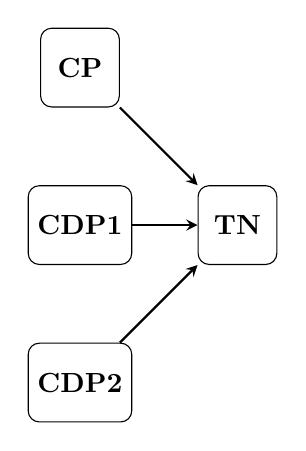
\begin{tikzpicture}[node distance=2cm]
						\node (cp1) [startstop] {\textbf{CP}};
						\node (cdp1) [startstop, below of=cp1] {\textbf{CDP1}};
						\node (cdp2) [startstop, below of=cdp1] {\textbf{CDP2}};
						\node (tn) [startstop, right of=cdp1] {\textbf{TN}};
						\draw [arrow] (cp1) -- (tn);
						\draw [arrow] (cdp1) -- (tn);
						\draw [arrow] (cdp2) -- (tn);
					\end{tikzpicture}
				\caption{Call answer diagram}
			\end{figure}

	\end{enumerate}

\section*{Problem 2}
	The solution is analogous to how IP addresses are assigned and used in
	networking. There are finite amount of IP addresses and they \textbf{can} be
	unique with an organization but \textbf{cannot} be unique across the globe.
	Hence, the concept of gateway is needed. For this problem, each organizations
	have its own gateway. Gateways could connect to each other based on a specific
	type of protocol and thus communicate with each other. Gateways take care of
	external communications across organizations. If an individual intends to
	communicate with another organization, it must go through the gateway.

\section*{Problem 3}
	Transmitting fax messages over the Internet, \newline
	\begin{addmargin}[1em]{1em}
		Advantage:
		\begin{itemize}
			\item Inexpensive
			\item Can reach anywhere the network is covered
		\end{itemize}
		Disadvantage:
		\begin{itemize}
			\item Proof of delievery cannot be obtained easily
		\end{itemize}
	\end{addmargin}

	Transmitting fax messages over the telephone network, \newline
	\begin{addmargin}[1em]{1em}
		Advantage:
		\begin{itemize}
			\item Proof of delievery can be obtained easily
		\end{itemize}
		Disadvantage:
		\begin{itemize}
			\item Distance matters
			\item Can get very expensive if long-distance faxing is needed
		\end{itemize}
	\end{addmargin}

\section*{Problem 4}
	\begin{enumerate}
		\item We know $\epsilon = \frac{d}{c}$, therefore,
			\begin{align*}
				\epsilon_{cb} &= \frac{\SI{10e-2}{meters}}{\SI{2.3e8}{meters\per\second}} \\
											&= \SI{4.347e-10}{seconds}
			\end{align*}
			Same formula applies, $\epsilon_{r} = \SI{4.347e-8}{}$,
			$\epsilon_{b} = \SI{4.347e-7}{}$,
			$\epsilon_{ma} = \SI{4.347e-4}{}$,
			$\epsilon_{c} = \SI{2.174e-2}{}$,
			$\epsilon_{s} = \SI{0.3134}{seconds}$.
		\item The answer is straighforward using $n = \frac{b}{t}$,
				\begin{addmargin}[1em]{1em}
					for circuit board,
					\begin{description}
						\item [at 10 kbps] $n = \SI{4.347e-6}{}$
						\item [at 1 Mbps] $n = \SI{4.347e-4}{}$
						\item [at 100 kbps] $n = \SI{4.347e-2}{}$
						\item [at 10 Gbps] $n = \SI{4.347}{}$
					\end{description}
					for room,
					\begin{description}
						\item [at 10 kbps] $n = \SI{4.347e-4}{}$
						\item [at 1 Mbps] $n = \SI{4.347e-2}{}$
						\item [at 100 kbps] $n = \SI{4.347}{}$
						\item [at 10 Gbps] $n = \SI{434.780}{}$
					\end{description}
					for building,
					\begin{description}
						\item [at 10 kbps] $n = \SI{4.347e-3}{}$
						\item [at 1 Mbps] $n = \SI{4.347e-2}{}$
						\item [at 100 kbps] $n = \SI{43.478}{}$
						\item [at 10 Gbps] $n = \SI{4347.800}{}$
					\end{description}
					for metropolitan area,
					\begin{description}
						\item [at 10 kbps] $n = \SI{4.348}{}$
						\item [at 1 Mbps] $n = \SI{434.78}{}$
						\item [at 100 kbps] $n = \SI{43478}{}$
						\item [at 10 Gbps] $n = \SI{4.347e6}{}$
					\end{description}
					for continent,
					\begin{description}
						\item [at 10 kbps] $n = \SI{217.4}{}$
						\item [at 1 Mbps] $n = \SI{21740}{}$
						\item [at 100 kbps] $n = \SI{2.174e6}{}$
						\item [at 10 Gbps] $n = \SI{2.174e8}{}$
					\end{description}
					for satellite,
					\begin{description}
						\item [at 10 kbps] $n = \SI{3130.4}{}$
						\item [at 1 Mbps] $n = \SI{313040}{}$
						\item [at 100 kbps] $n = \SI{3.1304e7}{}$
						\item [at 10 Gbps] $n = \SI{3.1304e9}{}$
					\end{description}
				\end{addmargin}
	\end{enumerate}
\end{document}
